\documentclass[12pt]{article}
\usepackage{graphicx}
\usepackage[utf8]{inputenc}
\usepackage[italian,english]{varioref}
\usepackage[greek,italian,english]{babel}
\usepackage{amsmath}
\usepackage{longtable}
\usepackage{wrapfig}
\usepackage{blindtext}
\usepackage{latexsym}
\usepackage{graphicx}
\graphicspath{{images/}}
\usepackage[style=authoryear, backend=biber]{biblatex}
\usepackage{caption}
\usepackage{subcaption}
\usepackage{csquotes}
\usepackage{amssymb}
\usepackage{physics}
\addbibresource{sample.bib}
\usepackage{epsf}
\pagenumbering{arabic}
\usepackage{imakeidx}
%\usepackage[T1]{fontenc}
\usepackage{geometry}
\geometry{a4paper,top=3cm,bottom=3cm,left=3.5cm,right=3.5cm,heightrounded,bindingoffset=5mm}
\usepackage{hyperref}

\begin{document}

	\begin{center}
	 
	
	\begin{figure}
		\centering
  		
\includegraphics[height=4.5cm]{unipd-bn.png}
	\end{figure}

	\vspace{20pt}

	\scshape{\Large{\bfseries{UNIVERSITÀ DEGLI STUDI DI PADOVA}}} \\
	\line(1, 0){350} \\
	\vspace{15pt}
	\scshape{\large{dipartimento di fisica e astronomia \\ "Galileo Galilei"
}} \\

	\vspace{45pt}
	\scshape{\large{laurea triennale in astronomia}}
	

	

	\vspace{50pt}
	
{\LARGE{\bfseries{Indagando le stelle di popolazione III }}} \\
	\vspace{25pt}
	\vspace{15pt}
	
		

	\vfill
	\begin{normalsize}
	\begin{flushleft}
	  \textit{Relatore} \hfill \textit{Laureando}\\
	  \vspace{1pt}
	  \textrm{Prof. Antonino Paolo Milone} \hfill \textrm{Roben Bhatti} \\	  Università di Padova \\
	  
	\end{flushleft}
	\end{normalsize}
	
	\vspace{20pt}
	\large{Anno accademico 2021/2022}
	
	\end{center}
	\vspace*{\fill}
\pagestyle{empty}	
\newpage
\
\pagestyle{empty}
\newpage

\tableofcontents
\newpage

\begin{abstract}

Le stelle più povere di metalli dell’alone galattico e delle galassie nane satelliti della Via Lattea offrono un'opportunità unica per fare luce sulle stelle di popolazione III.
 In questa tesi vengono presentate le principali tecniche di indagine ed i maggiori risultati.
  Molti di essi provengono da studi recenti di archeologia galattica in cui viene condotta  spettroscopia stellare ad alta risoluzione per ricavare le abbondanze chimiche delle stelle di bassissima metallicità.
  Vengono descritte le stelle più povere di metalli ad oggi note, e analizzati i due principali gruppi di stelle,  C-rich e C-poor, classificate sulla base del diverso contenuto di carbonio.
  Dal punto di vista teorico, la composizione chimica osservata delle stelle estremamente povere di metalli viene confrontata con quella che, secondo le simulazioni, corrisponde al materiale rilasciato da vari tipi di supernova. Tale confronto ci permette di risalire alle proprietà delle stelle di popolazione III, dalle cui ceneri si sono formate le stelle povere di metalli.
  La tesi include anche una discussione su dei metodi di indagine alternativi e complementari all'archeologia galattica, che si basano sull'investigazione dell'universo ad alto redshift.





\end{abstract}




\newpage
\section{Introduzione}
\label{introduzione}
Negli ultimi decenni lo studio delle stelle della Via Lattea ha fornito un potente strumento per analizzare la natura della nostra galassia, la sua struttura e le dimensioni. In particolare, tramite i profili di abbondanze chimiche è possibile scoprire indirettamente le stelle più antiche. L’assunzione implicita è che le stelle con la metallicità più bassa (dove con metallicità ci si riferisce a tutti gli elementi più pesanti del Litio) sono probabilmente le stelle più vecchie che conosciamo. La seconda assunzione, basata su studi teorici, è che le stelle e le galassie abbiano iniziato a formarsi a redshift z $\sim$ 20 - 30, circa 100 – 200 Myr dopo il Big Bang (\cite{Bromm}).

La cosmologia Near-field si basa sull’ipotesi che lo studio delle stelle nella Via Lattea ci possa dire le condizioni presenti nei primi miliardi di anni dal Big Bang. Il metodo si basa sullo stretto legame tra la massa di una stella e il suo tempo di vita; stelle molto massicce muoiono relativamente presto esplodendo in supernove mentre quelle poco massicce possono vivere anche miliardi di anni. Le popolazioni stellari contengono quindi informazioni sul passato dei sistemi che le ospitano, legando lo stato presente di una galassia alla sua storia evolutiva.
Quest’approccio richiede osservazioni dettagliate di singole stelle e quindi è più facile studiare la Via Lattea e le sue galassie nane satelliti.
Studiare la composizione chimica delle stelle è di fondamentale importanza perchè le loro atmosfere conservano informazioni sulle condizioni chimiche e fisiche delle nubi che le hanno generate. Negli ultimi decenni molteplici studi sono stati effettuati sulla ricerca delle stelle estremamente povere di metalli (bassissima metallicità) nell’alone della Via Lattea (\cite{Beers}); queste stelle permettono di indagare su una considerevole quantità di fenomeni legati alla natura dell’Universo primordiale, per questo ci si riferisce spesso a questo campo con il termine di “archeologia stellare”. Le stelle a bassa metallicità rivelano informazioni uniche sulla formazione delle prime stelle e le loro esplosioni in supernove, la loro evoluzione chimica, la formazione delle prime proto-galassie e il loro assemblaggio in galassie maggiori. Quest’ultimo approccio è nominato “archeologia delle galassie nane” perchè al posto delle stelle vengono studiate intere galassie nane che contengono stelle a bassa metallicità per ricavare i processi di formazione delle galassie stesse nell’universo primordiale (\cite{Frebel2012}).
Le stelle locali sono facilmente osservabili e offrono quindi un approccio alternativo alla cosmologia far-field ovvero ad uno studio ad alto redshift dell’universo.

\newpage
\subsection{Definizioni e concetti preliminari}
Prima di cominciare con la trattazione è necessario dare una serie di definizioni.
\paragraph{Abbondanze:}
L’abbondanza di un elemento A, $\varepsilon(A)$, è definita su scala logaritmica in termini del numero di atomi dell’elemento A, N$_A$, rispetto al numero di atomi di H, N$_H$:
\begin{equation}
  \log_{10} \varepsilon(A) = \log_{10} (N_A/N_H) + 12
\end{equation}

Dove il 12 è un valore costante. Per l’idrogeno $\log_{10}\varepsilon(H) =12$.
Solitamente ci si riferisce ad una "sovra-" abbondanza di un elemento quando è più alta rispetto a quella solare. 
Nella letteratura scientifica le abbondanze stellari solitamente sono presentate in termini dei loro valori rispetto a quelli solari:
\begin{equation}
[A/H] \equiv \log_{10}(N_A/N_H)_{\star} - \log_{10}(N_A/N_H)_{\odot}
\end{equation}

Per esempio $[Fe/H]=-4.0$ corrisponde ad un abbondanza di $10^{-4}$ rispetto a quella del sole. Diventa quindi importante sapere con precisione le abbondanze solari. Nelle stelle l’elemento più comune da misurare è il ferro vista la pletora di linee di assorbimento derivanti da transizioni associate a questo elemento. Storicamente ha assunto il ruolo di  riferimento per le comparazioni di metallicità di una stella con un'altra. 
\begin{equation}
[Fe/H] = \log_{10}(N_{Fe}/N_H)_{\star} - \log_{10}(N_{Fe}/N_H)_{\odot}
\end{equation}

 Da un punto di vista semantico le stelle povere di metalli non sono sinonimo di povere di ferro. Si vedrà che questo è vero per stelle con $[Fe/H]>-4.0$ ma sotto questo valore si riscontrano grandi quantità di carbonio o altri elementi rispetto al ferro. 
 
\paragraph{Assunzioni sui modelli atmosferici:} La radiazione continua emessa dalla fotosfera è soggetta ad una serie di assorbimenti e perciò le abbondanze chimiche stellari possono essere ricavate in diversi modi; il modello più semplice è quello monodimensionale (1D) che assume l’equilibrio idrostatico, la costanza del flusso, equilibrio termodinamico locale (LTE) e che tratta la convezione in termini di una semplice mixing length theory. I parametri atmosferici che definiscono il modello atmosferico sono la temperatura effettiva T$_{eff}$, la gravità superficiale $\log$ g e la composizione chimica [M/H], (dove M sta per metalli). 
La temperatura effettiva viene definita come la temperatura che un corpo nero ha per irradiare nell'unità di tempo e di superficie la quantità di energia emessa in un secondo e nell'unità di area dalla fotosfera stellare. Questa diventa simile alla temperatura reale della stella quando la sua curva di emissione è altrettanto simile a quella di corpo nero. La temperatura effettiva è definita da:
 \begin{equation}
  L\star=4\pi R^{2}\sigma T^{4}_{eff}
\end{equation}
dove $\sigma$ è la costante di Boltzmann, $L_\star$ è la luminosità della stella e R il suo raggio. Tuttavia la misura del raggio è complicata e si preferisce stimare la temperatura di colore usando l'indice di colore, ovvero la differenza tra le magnitudini apparenti in due diverse bande fotometriche.
La gravità superficiale di una stella è l'accelerazione gravitazionale di cui è affetta una particella posta sulla superficie. Tipicamente è espressa in scala logaritmica:
\begin{equation}
  \log(g)\quad \textit{con} 	\quad g=g_\odot \frac{M}{R^2}
\end{equation}
La gravità superficiale è un parametro importante da considerare insieme alla temperatura perché varia l'equilibrio di ionizzazione secondo la formula di Saha. \\ Inoltre c'è da considerare anche la velocità di microturbolenza che influisce sull'allargamento delle righe.
Dati questi parametri si confronta il flusso teorico con quello osservato e si ottiene un best-fit che rappresenti la stella osservata, da questo si ricavano le abbondanze del modello che sono dunque quelle della stella osservata.

Altri modelli più sofisticati sono quelli tridimensionali 3D LTE/NLTE (non-LTE) più rigorosi e realistici. La differenza tra i due modelli LTE/NLTE e 1D/3D è $\sim 0.5-1$ dex, la sovrastima risulta generalmente con il modello 1D/LTE. La figura \ref{1d3d} mostra la differenza di abbondanze tra [X/Fe](3D) – [X/Fe](1D) vs il numero atomico. Si notano le estreme differenze per C, N e O.
In genere il modello 3D mostra le disomogeneità delle temperature che aumentano con la metallicità e quindi le differenze con i modelli 1D si ampliano.

 In generale dove possibile si preferiscono utilizzare le abbondanze ricavate con i modelli 3D/NLTE. Tuttavia in questo elaborato, se non specificato, ci si riferisce ad abbondanze ricavate con modelli 1D/LTE che sono disponibili per un maggiore campione di stelle e quindi è più affidabile elaborare un trend. É incauto mescolare abbondanze ricavate da modelli 1D con modelli 3D quando si deve elaborare una tendenza, soprattutto con stelle che hanno composizioni anomale come in questo caso.

\begin{figure}[htp!]
\center
  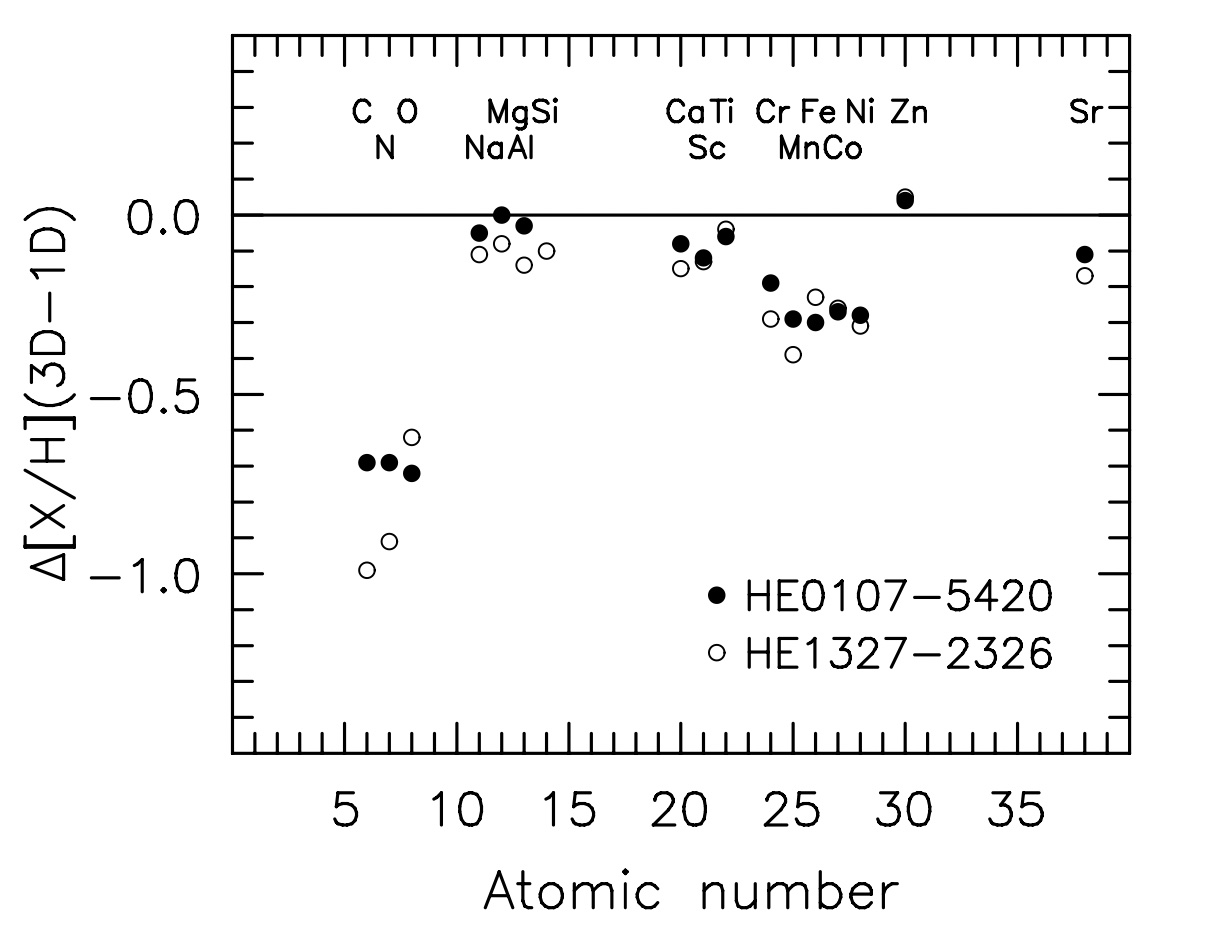
\includegraphics[width=
0.8 \textwidth]{1d3d}
  \caption{La differenza in abbondanze $[X/Fe]_{3D}$ – $[X/Fe]_{1D}$ contro il numero atomico basata su modelli atmosferici monodimensionali e tridimensionali per due tra le stelle più povere di metalli conosciute HE 1327–2326 e HE 0107–5240, entrambe con $[X/Fe]_{1D} \sim -5.5$. \cite{Frebel_2013}  }
  \label{1d3d}
\end{figure}



\newpage
\
\newpage


\section{Archeologia stellare}

L’archeologia stellare, come accennato nella sezione \ref{introduzione}, si occupa di studiare il modo in cui le stelle si formano e evolvono tramite l’analisi delle abbondanze chimiche delle stelle vecchie. I parametri che vengono utilizzati in questo ambito sono le distribuzioni spaziali, cinematiche e le età delle stelle in oggetto. Nel contesto cosmologico siamo interessati allo studio delle prime stelle che si sono formate nel primo miliardo di anno dopo il big bang, l’età di queste stelle è di fondamentale importanza; tuttavia ricavare questo parametro è complicato, quindi è necessario usare informazioni complementari. 
Prima però è necessario indagare la struttura della nostra galassia per capire dove cercarle.

\subsection{La Via Lattea}

\paragraph{Le componenti}
\label{componenti}
La via Lattea, in figura \ref{galassia}, è formata da diverse componenti osservabili direttamente, le più note sono: il disco, il bulge e l’alone.
Il disco racchiude gran parte della componente stellare e gassosa e a partire dagli ’80 si è diffusa l’idea di una sua natura duale (\cite{Yoshii}); è caratterizzato da una componente sottile e una spessa che è verticalmente più estesa. Le stelle giovani e ad alta metallicità, dette di popolazione I, sono principalmente collocate nel disco sottile, con una metallicità media di [Fe/H] $\sim$ - 0.2; nella componente spessa del disco si distingue una parte dove la metallicità media è [Fe/H] $\sim$  - 0.6 e un’altra con metallicità più bassa - 2.5 $<$ [Fe/H] $<$ - 1.0. Si nota che gli ammassi aperti più poveri di metalli si trovano nelle regioni esterne mentre quelli più metallici e più vecchi sono nelle zone più interne e ciò indica l’esistenza di un gradiente di metallicità. La natura duale del disco ha permesso la formulazione di numerose ipotesi sulla sua natura, tra queste si pensa che le stelle più povere di metalli si siano spostate in alto verticalmente mentre sul piano galattico si sono formate stelle più giovani.
Il bulge è stato tra le prime componenti della galassia ad essersi formato e per cui si ipotizza contenere le stelle più povere di metalli ma per vari motivi è un territorio difficile da analizzare. Il bulge, oltre alle stelle vecchie, contiene diverse popolazioni di stelle giovani il che comporta una difficoltà ulteriore nell’isolamento delle stelle di interesse, inoltre l’ambiente è molto denso e la grande quantità di polveri presenti rende ancora più complicato osservare questa componente. 

L’alone ha una distribuzione sferica che si sviluppa intorno al disco e racchiude il bulge estendendosi fino a 150 kpc. Contiene generalmente stelle più vecchie e povere di metalli. Le metallicità medie per la componente interna e esterna sono [Fe/H]$<$ - 1.6 e - 2.2 rispettivamente fino ad arrivare alla stella più povera di metalli conosciuta fino ad ora, la stella di \cite{keller} con metallicità inferiore a [Fe/H] = - 7.3.
Le distribuzioni spaziali, cinematiche e di abbondanze chimiche delle stelle dell’alone mostrano che esso sia formato da sotto-strutture probabilmente risultanti da eventi di accrescimento.  In genere l’alone è descritto in termini di una componente interna che potrebbe essersi formata direttamente durante l’evoluzione della galassia e una componente esterna più diffusa formatasi da eventi passati di accrescimento e distruzione mareale delle galassie nane. 

\paragraph{Le galassie nane satelliti}

La nostra galassia è circondata da diverse galassie nane che orbitano nell’alone esterno. Le più massicce sono le nubi di Magellano, due galassie irregolari caratterizzate da un alto tasso di formazione stellare. Inoltre sono presenti galassie nane sferoidali (DSph) e galassie ultra-faint. Quest’ultime sono di primaria importanza perché ospitano popolazioni di stelle estremamente povere di metalli e quindi informazioni chiave sulla formazione delle stesse. Negli ultimi anni, studi mostrano come la formazione della Via Lattea sia strettamente connessa alla natura e alla storia delle DSph, che potrebbero essere state i mattoni fondamentali della sua costruzione. 


\paragraph{L'alone di materia oscura}

Alla Via Lattea è associato un alone di materia oscura che si estende fino a 300\,kpc dal centro e con una massa tra $1.0 – 2.4 \cdot 10^{12} $ M$_{\odot}$. 
La comprensione di tale alone e' di fondamentale importanza in astrofisica in quanto geometria stessa e l'evoluzione dell’Universo sono determinate dalle proprietà della materia oscura e dal loro legame con la materia barionica. \\

I primi modelli teorici di formazione stellare (\cite{Abel}) prevedevano una funzione di massa dominata dalle stelle di grande massa ($\sim$100 M$_{\odot}$) per le stelle di popolazione III. Tali grandi masse le renderebbero inosservabili oggi, dato il loro tempo di vita relativamente breve, di qualche decina di milione di anni.
Studi teorici più recenti (\cite{Stacy}) suggeriscono invece che queste stelle di popolazione III potrebbero essere meno massicce ed alcune di esse potrebbero avere masse paragonabili a quella solare. Nell'ambito di questi scenari, le stelle di popolazione III sono osservabili ancora oggi e ci aspetteremmo di trovarle  principalmente nell’alone e nel bulge della Via Lattea.


\begin{figure}[htp!]
\center
  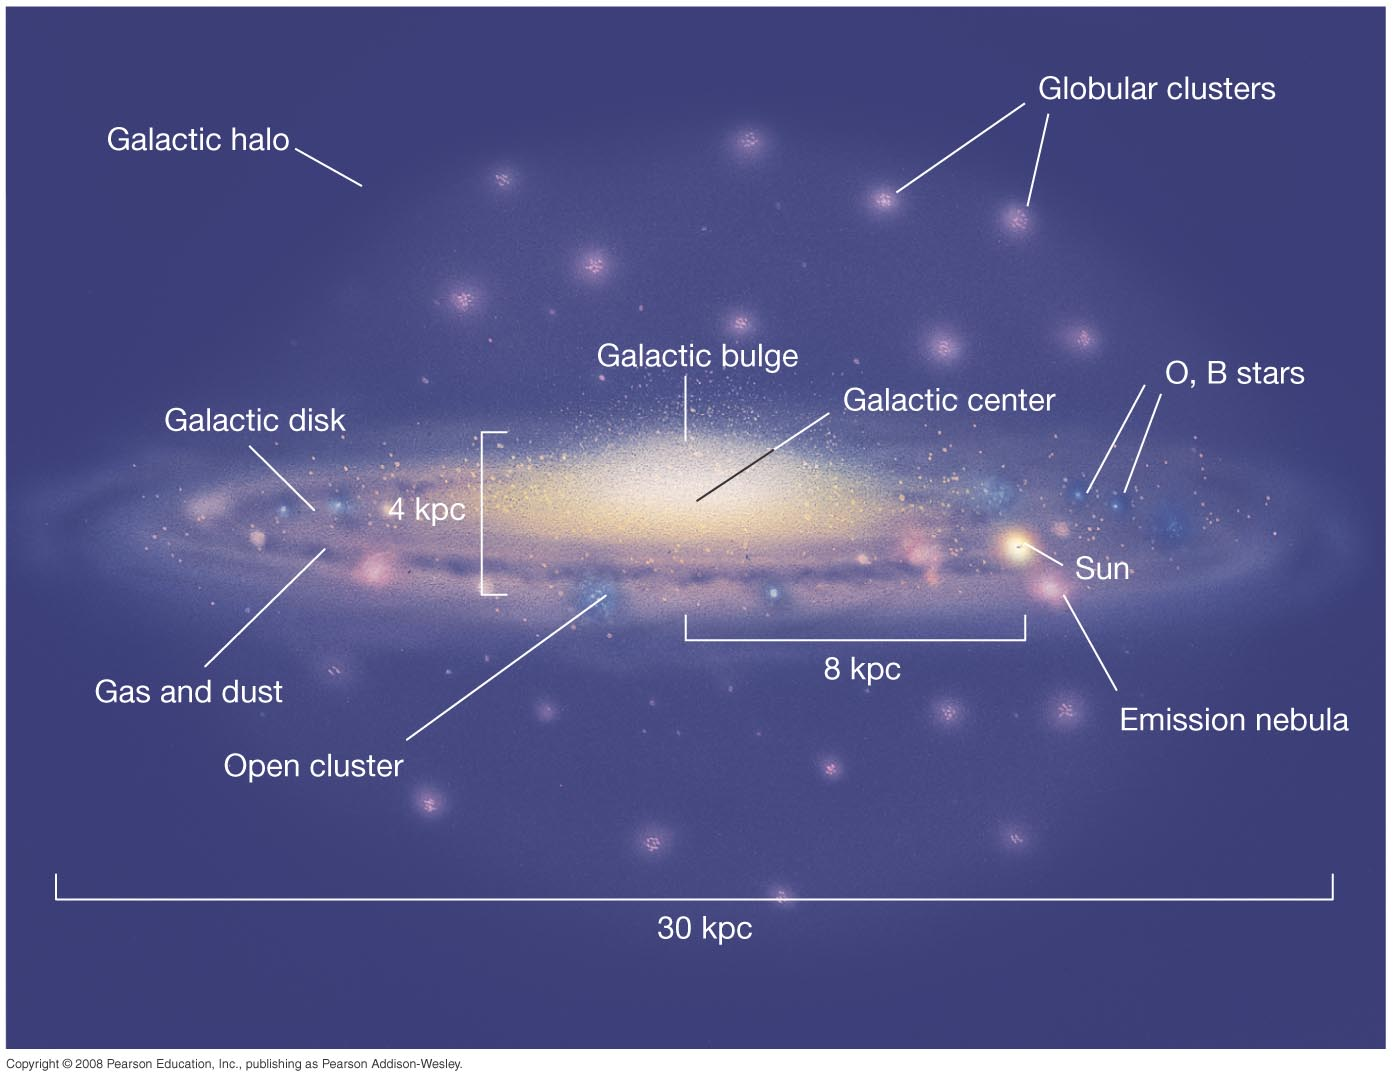
\includegraphics[width=
0.8 \textwidth]{galassia}
  \caption{immagine schematica della Via Lattea. }
  \label{galassia}
\end{figure}
\
\newpage
\subsection{La ricerca delle stelle più povere di metalli}
\

\paragraph{Il ruolo delle abbondanze chimiche}

Nei primi minuti dopo il Big Bang l’universo era formato solo da idrogeno, elio e litio, tutti gli altri elementi (tranne il berillio e il boro) sono stati prodotti successivamente nelle stelle e nelle esplosioni delle supernove. L’assunzione su cui si basa l’archeologia stellare è che le prime stelle a formarsi abbiano avuto una metallicità estremamente bassa o addirittura nulla. Quindi le stelle più povere di metalli sono le migliori candidate per studiare i primi eventi di formazione stellare. Le due zone più accessibili sono l’alone galattico e le galassie nane satelliti della Via Lattea, tuttavia il posto teoricamente migliore per cercare le prime stelle è il bulge ma come discusso nella sezione \ref{componenti} è una zona estremamente complicata da osservare.

\paragraph{Metodi di indagine}

Decenni di ricerche hanno mostrato che le stelle più povere di metalli sono rare, localmente ci si aspetta di trovarne una ogni 100 000 stelle campionate. Numerose tecniche sono state utilizzate per migliorare le possibilità di trovare queste stelle nell’alone galattico. Alcune di queste sono:
\begin{itemize}
\item \textbf{Indagini sull’elevato moto proprio}: una grande frazione delle stelle dell’alone hanno un moto proprio elevato rispetto a quelle del disco galattico. La prima stella con [Fe/H] $<-3.0$ (G64-12) è stata trovata utilizzando questo metodo nel 1981 da \cite{1981}. Altre indagini sono state fatte negli anni 90’ e sono state trovate in tutto una decina di stelle con [Fe/H] $<$ - 3.0. Più recentemente la missione GAIA dell’ESA fa parte di questo tipo di indagini. 
\item \textbf{Indagini con il prisma obbiettivo Schmidt}: questo tipo di prisma permette di ottenere spettri a bassa risoluzione (R = $\lambda/\Delta\lambda$ $\sim$ 400) per un grande numero di stelle simultaneamente. L’analisi della profondità della riga Ca II a 3933.6 $\r{A}$ rispetto alle righe dell’idrogeno o il colore della stella portano ad una prima cernita delle possibili stelle povere di metalli. Fino ad ora questo è stato il metodo più proficuo per trovare le stelle a bassa metallicità.

\item \textbf{Indagini spettroscopiche}: Lo Sloan Digital Sky Survey (SDSS) e il seguente SEGUE hanno scandagliato spettroscopicamente il cielo con un potere risolutivo di R $\sim$ 2000 e si sono dimostrati un potente strumento di indagine.
\item \textbf{Indagini fotometriche}: Sistemi fotometrici vengono utilizzati come potente alternativa agli spettri a bassa risoluzione per trovare delle stelle candidate. Per esempio nel sistema UBV l’eccesso ultravioletto (dato dalla sensibilità nella banda U delle righe spettrali del ferro) è utilizzato per ottenere stime sulla metallicità senza passare prima per uno spettro. Una survey di questo tipo attualmente in corso è la SkyMapper Southern Sky Survey il cui filtro è disegnato appositamente per determinare i parametri atmosferici delle stelle povere di metalli. Questa survey ha permesso di scovare la stella più povera di metalli conosciuta, la stella di \cite{keller} con [Fe/H] $<$ - 7.3 nel 2014.


\end{itemize}

Quindi il primo passo consiste nello scandagliare il maggior numero di stelle possibile con metodi a bassa risoluzione per trovare i candidati migliori.
Il secondo consiste nell’ottenere uno spettro ad alta risoluzione (R $>$ 30000), alto S/N delle candidate. Questi spettri vengono utilizzati per determinare le abbondanze chimiche, i rapporti isotopi e in alcuni casi le età stellari. La maggior parte delle abbondanze chimiche si ottengono tramite la larghezza equivalente (EW) delle righe di assorbimento con un incertezza $\sigma$(EW) associata di FWHM$^{0.5}$/(S/N), dove FWHM è la larghezza a metà altezza della linea. Incrementando il potere risolutivo dello spettrografo insieme al rapporto segnale rumore l’incertezza associata diminuisce, permettendo di rilevare righe sempre più deboli. Ciò è di fondamentale importanza per rilevare le righe estremamente deboli delle stelle povere di metalli. 


\subsection{Le stelle più povere di metalli conosciute}
\label{povere}
\begin{figure}[htp!]
\center
  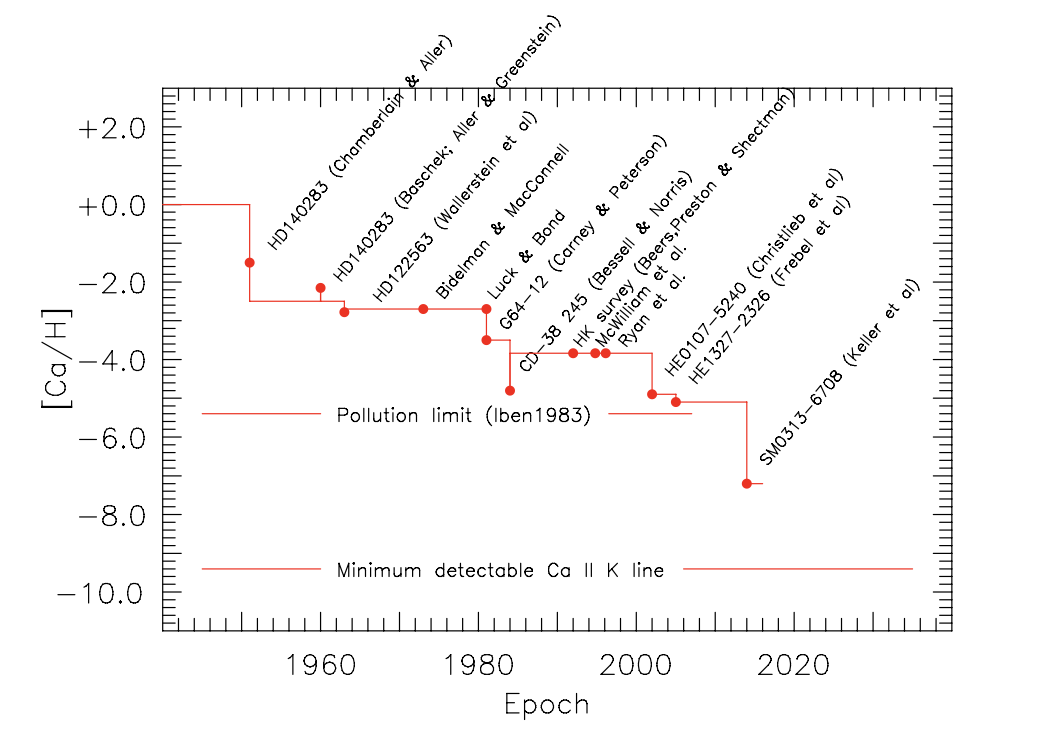
\includegraphics[width=0.9 \textwidth]{epoch}
  \caption{ L’abbondanza di calcio [Ca/H] per le stelle più povere di metalli conosciute all’epoca in funzione dell’anno in cui sono state scoperte. Si usa il calcio perché a basse metallicità è ancora osservabile a differenza del ferro. I cerchi rappresentano i valori delle abbondanze determinati dagli autori all’epoca mentre le linee sono i valori moderni accettati. Si notano i limiti di Iben e Frebel $\&$ Norris. Figura tratta da \cite{principale}}
  \label{epoch}
\end{figure}
\



Nella figura \ref{epoch} sono mostrate alcune delle stelle più povere di metalli scoperte in funzione dell’anno in cui sono state scoperte e dell’abbondanza di [Ca/H]. 
Una stella non può scendere, per ragioni tecniche o fisiche, sotto due limiti inferiori: il limite di Iben e quello di Frebel $\&$ Norris.
Il limite di Iben è pari a [Ca/H] = - 5.4 (assumendo [Ca/Fe] = 0.3) e si trova calcolando la probabile abbondanza superficiale che una stella con metallicità nulla, avrebbe acquisito per accrescimento dal mezzo interstellare nel corso di 10 miliardi di anni, assumendo una metallicità di accrescimento di [Fe/H] = - 0.6 mediata nel tempo. Tuttavia non deve sorprendere di trovare stelle con una metallicità inferiore data la natura grossolana di questa stima.  Il limite di Frebel $\&$ Norris, invece, è più restrittivo e si basa sul limite inferiore di 20 m$\r{A}$ dell’assorbimento della riga CaII K di una ipotetica gigante rossa a bassa metallicità con parametri atmosferici di T$_{eff}$=4500K e $log\ g$ = 0.5. La riga del CaII K è la riga più forte nello spettro di una stella povera di metalli e la sua forza è intrinsecamente maggiore nelle giganti rosse che nelle nane della sequenza principale. Il limite di Frebel $\&$ Norris è pari a [Ca/H] = - 9.4. Straordinari progressi sono stati fatti negli ultimi due decenni da un punto di vista osservativo e siamo arrivati probabilmente ad un punto in cui un ulteriore progresso richiederà molto più tempo. Lo spettro della stella più povera di metalli scoperta, la stella di Keller, ha una metallicità stimata di [Fe/H] $<$ - 7.2 e nessuna riga del Ferro è stata osservata. Gli unici altri elementi rilevati sono Li, C, Ca e Mg mentre la forza della riga CaII K è di soli 90 m$\r{A}$. 

\paragraph{La stella di Keller}
Lo spettro ad alta risoluzione (R = 28,000)  della stella d’alone “SMSS J031300.36-670839.3” figura \ref{keller}  mostra come le righe del ferro sono completamente assenti. Infatti è possibile stimare solo un limite superiore dell’abbondanza di ferro con un intervallo di confidenza 3$\sigma$: [Fe/H] $<$  -7.2, il più basso mai stimato. La debolezza delle righe di assorbimento permette di derivare solo l’abbondanza di quattro elementi: [Ca/H] = -7.0, [Mg/H] = -3.8, [C/H] = -2.6 e [Li/H] = 0.7 . La gigante rossa è stata scoperta grazie alle indagini di Skymapper che con il suo speciale filtro ha permesso di trovare parametri atmosferici di T$_{eff}$ = 5125 K e log g = 2.3. 
L’abbondanza di litio, A(Li) = 0.7, è molto inferiore a quella associata al gas primordiale A(Li) = 2.72. Ci si aspetta un tale livello di litio in una gigante rossa povera di metalli a causa del circolo di materiale nelle regioni ad alta temperatura dove il litio viene distrutto e diluito nell’inviluppo convettivo.
I modelli di evoluzione chimica galattica, che considerano una bassa energia di esplosione delle supernove di popolazione III, mostrano che la sua formazione sia avvenuta solo in seguito ad un singolo evento di supernova a redshift 25 $<$ z $<$ 17. \cite{keller} hanno comparato le abbondanze di SMSS J031300.36-670839.3 con quelle di diversi modelli di nucleosintesi delle supernove di popolazione III variando parametri come la massa della progenitrice, l’ energia di esplosione e il mescolamento interno. Il miglior modello, figura \ref{keller2}, prevede un’energia di esplosione di 1.8x10$^{51}$ erg relativa a una stella di 60M$_{\odot}$ con una piccola quantità di mescolamento dovuta all’espulsione di materia a causa di instabilità di Rayleigh-Taylor. 
In questo modello si forma un buco nero nel quale il nucleo della stella massiccia viene assorbito. I metalli che vengono sintetizzati durante la vita della stella vengono intrappolati nel buco nero mentre gli elementi più leggeri che sono situati a raggi maggiori sono dispersi nell’esplosione. 
Lo spettro della stella di Keller esclude progenitrici fuori dal range 10-70 M$_{\odot}$, infatti supernove inferiori a 10 M$_{\odot}$ rilasciano grandi quantità di ferro, mentre quelle maggiori di 70M$_{\odot}$ non producono un eccesso di carbonio e rilasciano grandi quantità di azoto. 

\begin{figure}[htp!]
\center
  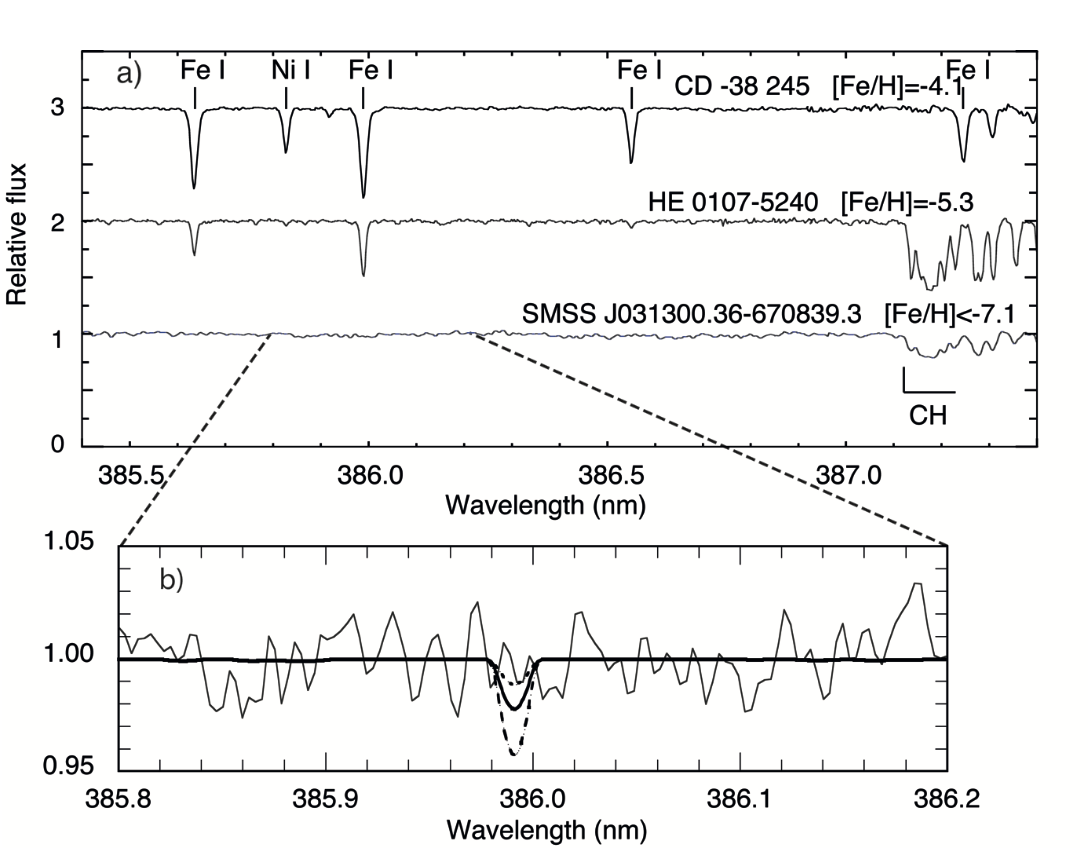
\includegraphics[width=1 \textwidth]{keller}
  \caption{Comparazione dello spettro della stella di Keller rispetto ad altre stelle povere di metalli. Lo spettro mostra la totale assenza delle righe del ferro ed è dominato dalla righe molecolari del CH. Sono sovrapposti gli spettri sintetici per [Fe/H]=-7.5, -7.2 (linea continua) e - 6.9. 
 }
  \label{keller}
\end{figure}
\


\paragraph{La stella di Nordlander}
\cite{nordlander} hanno riportato la scoperta di SMSS J160540.18-144323.1 nonché la stella più povera di metalli identificata fino ad ora, con una metallicità pari a [Fe/H] = - 6.2 $\pm$ 0.2  (1D LTE). La gigante rossa è ricca di carbonio [C/Fe] = 3.9 $\pm$ 0.2 e sono stati identificati anche Mg, Ca, e Ti. La stella è stata scoperta grazie al progetto Skymapper per la ricerca delle stelle estremamente povere di metalli. Skymapper usa filtri sensibili alla metallicità per effettuare una prima indagine a media risoluzione (R=3000) che ha confermato una metallicità di [Fe/H] $<$ - 5 . Lo spettro ad alta risoluzione (R=28000), figura \ref{nordlander}, è stato acquisito dal Magellan Clay telescope.
Usando i modelli di supernove di popolazione III, di Heger $\&$ Woosley si trova un risultato compatibile solo per progenitori di piccole masse M $\sim$ 10 M$_{\odot}$ con basse energie di esplosione $<10^{51}$ erg. Modelli che considerano range di massa diversi non riproducono un' elevata abbondanza di carbonio come quella osservata, figura \ref{nordlander2}. \\ Le figure \ref{keller2} e \ref{nordlander2} sono approfondite nella sezione \ref{limiti}.



\begin{figure}[htp!]
\center
  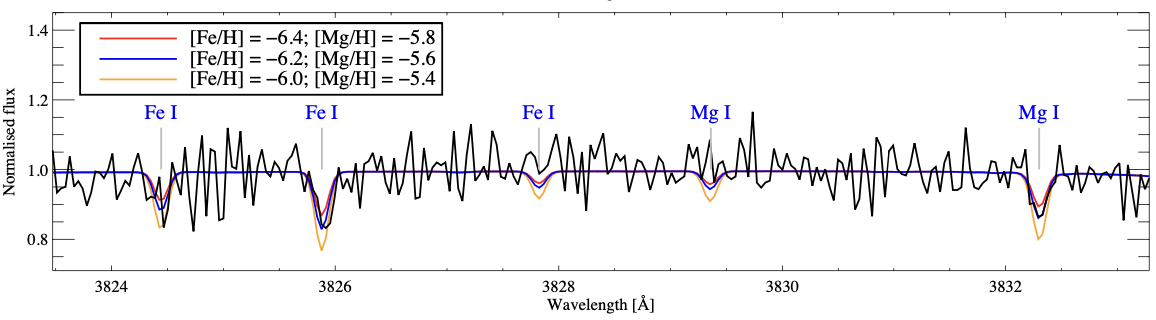
\includegraphics[width=1 \textwidth]{nordlander}
  \caption{Spettro ad alta risoluzione (MIKE) della stella di Nordlander e fit delle righe Fe, Mg per tre modelli indicati in alto a sinistra. }
  \label{nordlander}
 \end{figure}



\begin{figure}[!tbp]
  \centering
     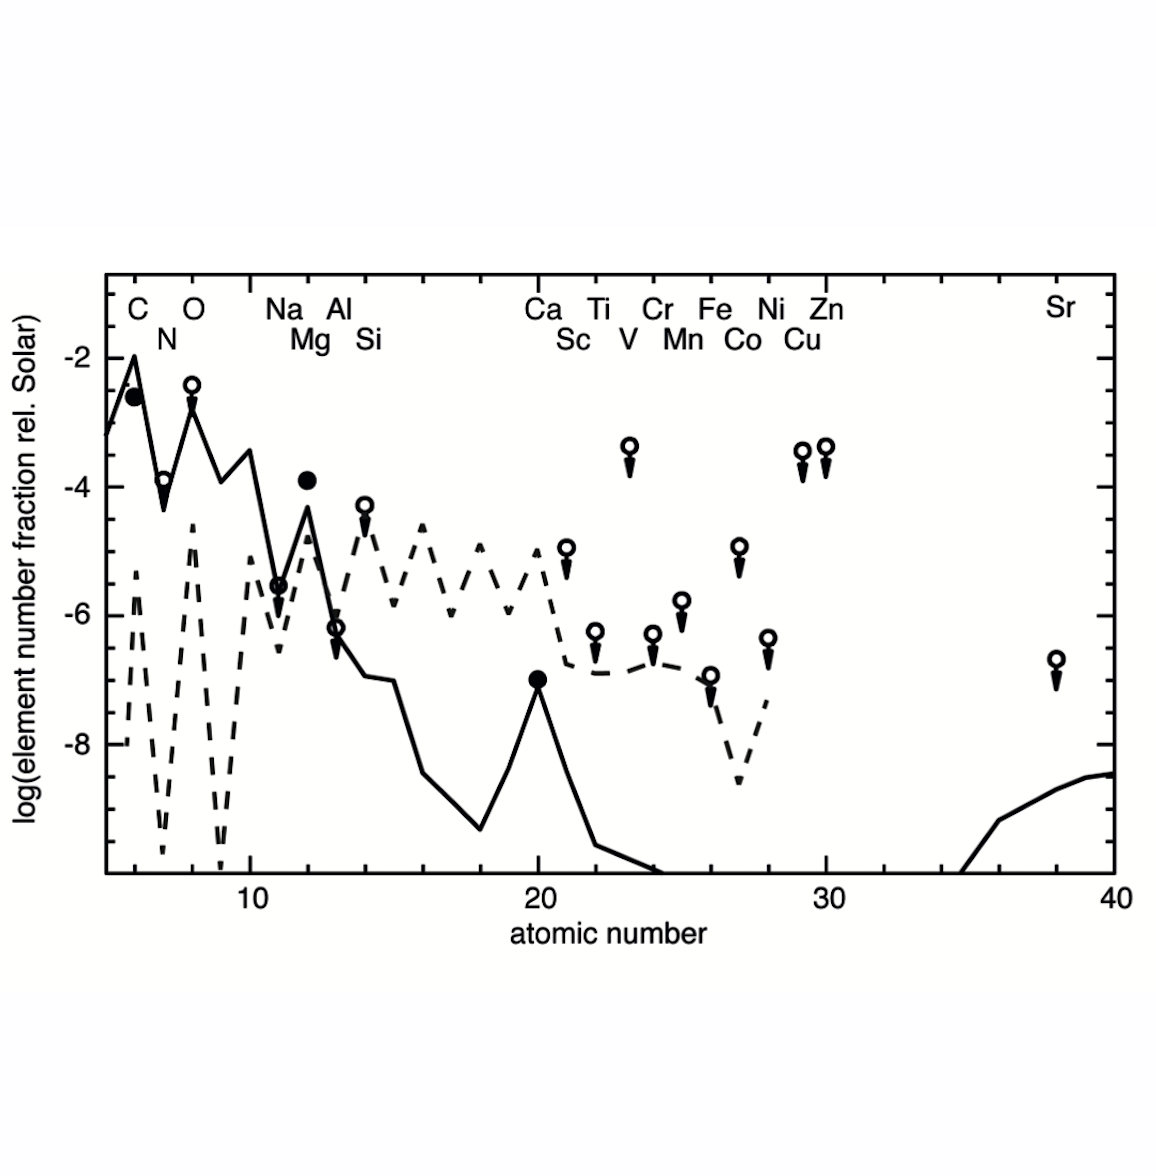
\includegraphics[width=0.6\textwidth]{keller2}
    \caption{Pattern di abbondanza per SMSS J031300.36-670839.3: le abbondanze determinate sono mostrate con cerchi mentre i limiti superiori 3$\sigma$ stimati a causa della debolezza delle righe sono segnati come cerchi aperti. La linea continua mostra le abbondanze prodotte da un modello di popolazione III di 60 M$_{\odot}$ per una bassa energia di esplosione e un basso livello di mescolamento interno. La linea tratteggiata mostra il modello di un esplosione di 200M$_{\odot}$.}
    \label{keller2}
  \end{figure}

  \
\begin{figure}[!tbp]
\centering

    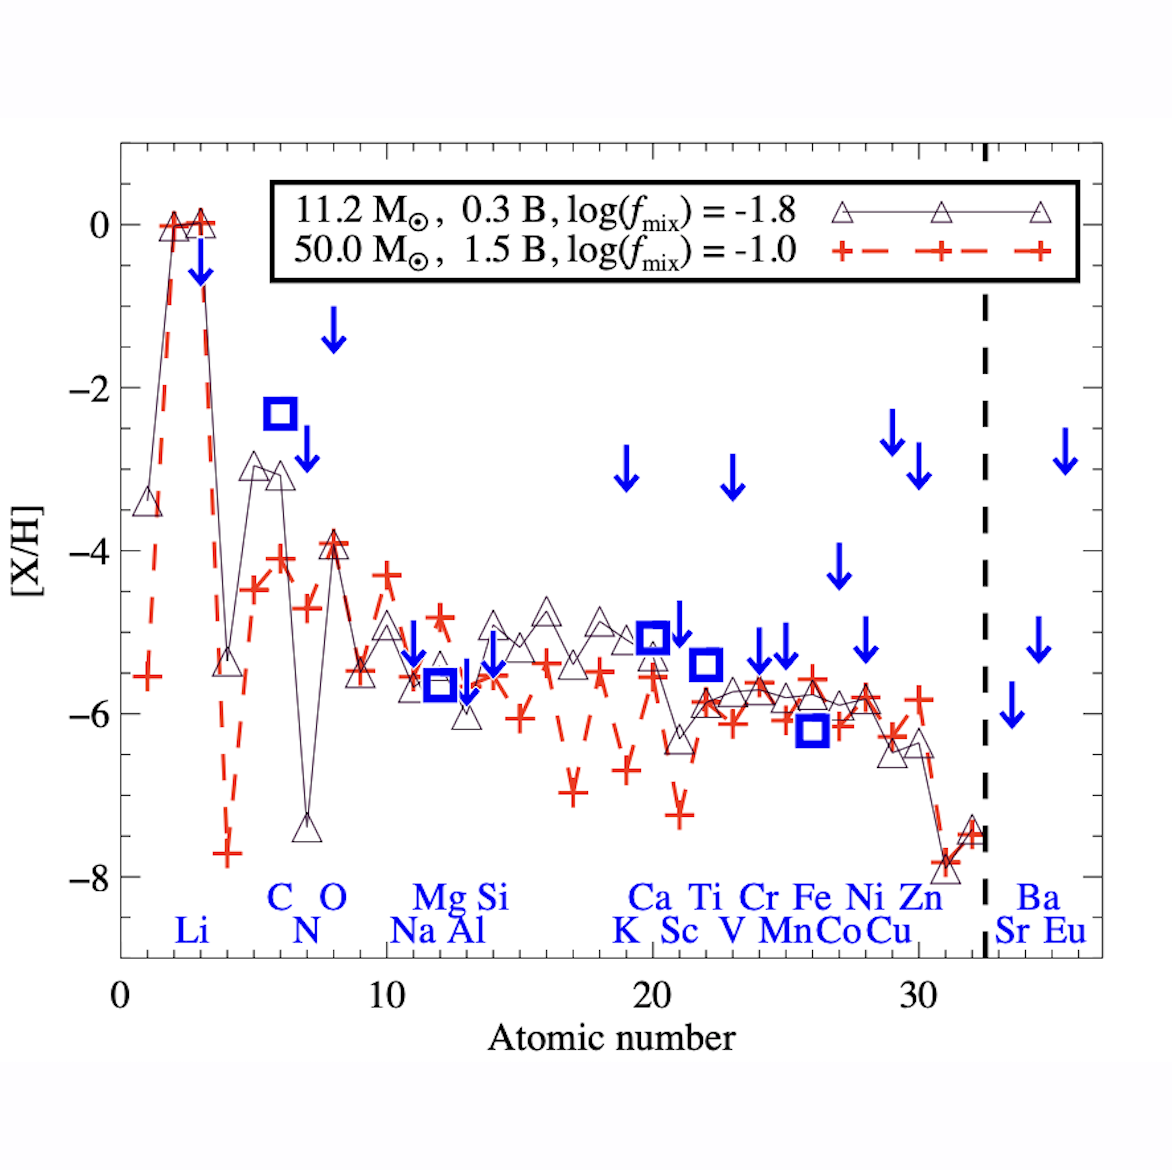
\includegraphics[width=0.7\textwidth]{nordlander2}
    \caption{Comparazione delle abbondanze misurate (quadrati blu) e limiti superiori 3$\sigma$ (frecce blu) con due modelli di esplosione di supernove: $\sim$ 10 M$_{\odot}$ e 50 M$_{\odot}$  rispettivamente linea continua nera e linea tratteggiata rossa. 
}
    \label{nordlander2}
 
\end{figure}

\newpage

\subsection{Popolazioni C-rich e C-normal per [Fe/H] $<$ -3.0}

\label{abbondanze1}

Nelle stelle povere di metalli ci sono diversi gruppi di elementi chimici raggruppati in base al loro principale meccanismo di produzione: gli elementi $\alpha$ (Mg, Ca, Ti) sono prodotti durante vari stadi di bruciamento nelle ultime fasi dell’evoluzione stellare, prima ma anche durante l’esplosione da supernova. Gli elementi ferrosi (23 $<$ z $<$ 30)  sono sintetizzati in molte zone di nucleosintesi come prima e durante l’esplosione, durante il decadimento radioattivo di nuclei pesanti o la diretta sintesi negli stadi di bruciamento esplosivi. Gli elementi leggeri e pesanti a cattura neutronica (z $>$ 38) sono prodotti nel processo s (slow) nelle stelle AGB, poi depositati nell’ISM tramite vento stellare o trasferiti ad una compagna binaria, oppure nel processo r (rapido) che avviene durante il collasso del nucleo in supernova. Le abbondanze osservate nelle stelle più povere di metalli sono state riprodotte con successo da modelli di supernove da stelle di popolazione III. 
I pattern di abbondanze di elementi del processo r, in particolare per z $>$ 56, sono straordinariamente allineati per tutte le stelle in cui avviene questo processo. Questo comportamento suggerisce l’universalità del processo r e porta agli stessi tassi di abbondanze sia nell’universo primordiale che a epoche successive. Questo permette di definire le condizioni dei modelli teorici del processo r ma anche di calcolare i tassi per gli elementi radioattivi come il torio e l’uranio e compararli con il materiale stellare rimasto, il che permette di datare queste stelle antichissime. Tuttavia un' impronta pulita del processo r può essere osservata solo per le stelle che si sono formate prima che il processo s sia potuto iniziare poiché ci sono delle deviazioni del processo r per gli elementi più leggeri prodotti nei processi a cattura neutronica. \\

Una delle scoperte più interessante per le stelle povere di metalli ([Fe/H] $<$ -3.0) è l’alta incidenza di stelle con un' abbondanza elevata di [C/Fe], ciò ha richiesto una classificazione ulteriore per stelle [C/Fe]$>$+0.7 in sottoclassi “Carbon Enhanced Metal Poor” (CEMP/ C-rich) sulla base delle abbondanze degli elementi derivati dalla cattura neutronica: CEMP-s (accrescimento dal processo s), CEMP-r (accrescimento dal processo r), CEMP-r/s (accrescimento da entrambi i processi) e CEMP-no (accrescimento non derivante da processi slow o rapid). La sottoclasse CEMP-s rappresenta la gran parte della popolazione C-rich. Queste stelle sono tuttavia estremamente rare sotto [Fe/H] = -3.0 quindi in questa discussione si escludono insieme alle CEMP-r/s e le CEMP-s, entrambe con [Fe/H] $>$ -3.0. 

\begin{figure}[htp!]
\center
  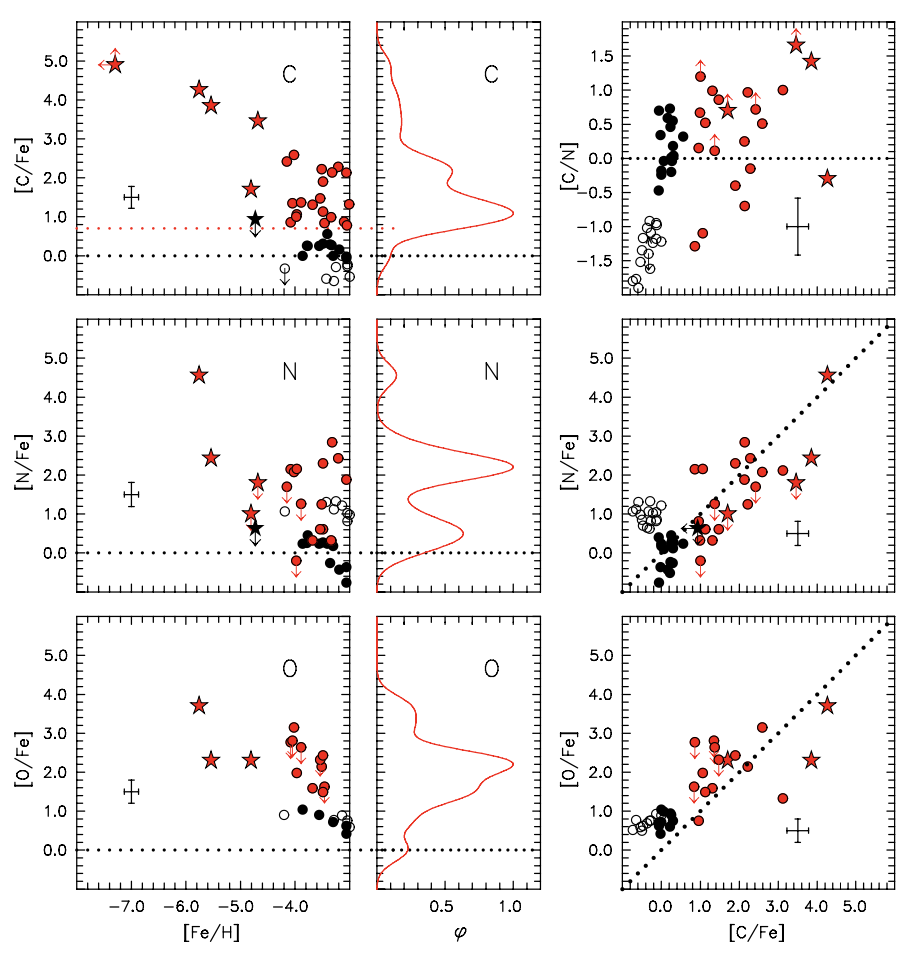
\includegraphics[width=0.8 \textwidth]{cno}
  \caption{[C/Fe], [N/Fe] e [O/Fe] in funzione di [Fe/H] (a sinistra) e [C/Fe] (a destra). I cerchi rossi e neri sono rispettivamente stelle  C-rich (escluse CEMP-s, CEMP-r e CEMP-r/s) e stelle C-normal. Cerchi se gli oggetti sono sopra [Fe/H] = - 4.5 e stelle se sotto. Le figure centrali rappresentano gli istogrammi generalizzati delle abbondanze a sinistra.  La linea rossa tratteggiata è il limite tra le stelle C-rich e C-normal fissato a [C/Fe]= +0.7.
 }
  \label{cno}
 \end{figure}
\



La figura \ref{cno}, tratta da \cite{principale}, mostra le distribuzioni di C,N,O in funzione di [Fe/H] e [C/Fe] per stelle nel range -8.0 $<$ [Fe/H] $<$ -3.0. i simboli neri rappresentano le stelle C-normal e i simboli rossi sono per le stelle C-rich.
I pannelli a sinistra mostrano [C/Fe], [N/Fe], e [O/Fe] in funzione di [Fe/H], al centro gli istogrammi normalizzati delle abbondanze di questi elementi nelle stelle C-rich e infine a destra [C/N], [N/Fe] e [O/Fe] in funzione di [C/Fe].
Si notano sovrabbondanze di ossigeno (rispetto al carbonio) nelle stelle C-rich in cui l’elemento è stato misurato. Questo è un risultato parziale perché le abbondanze di O non sono disponibili per molte delle stelle in figura a causa della maggior difficoltà nel misurarle. Per l’azoto invece si riscontrano sia stelle con grandi sovrabbondanze che con poche e i suoi istogrammi suggeriscono una distribuzione bimodale. 
Questo comportamento delle stelle C-rich è in contrasto con le giganti rosse C-normal (cerchi neri vuoti e pieni) dove si nota un comportamento bimodale nei pannelli relativi a C e N, molto evidente in quello in alto a destra. \cite{spite} mostrano che questo effetto è dato dal mescolamento dalle regioni interne a quelle più esterne di materiale derivante dai processi del ciclo CN nelle RGB.
Nelle stelle C-rich, che comprendono sia giganti che nane, le sovrabbondanze di C, N e O sono indicative di ulteriori processi oltre al ciclo CN. 


\begin{figure}[htp!]
\center
  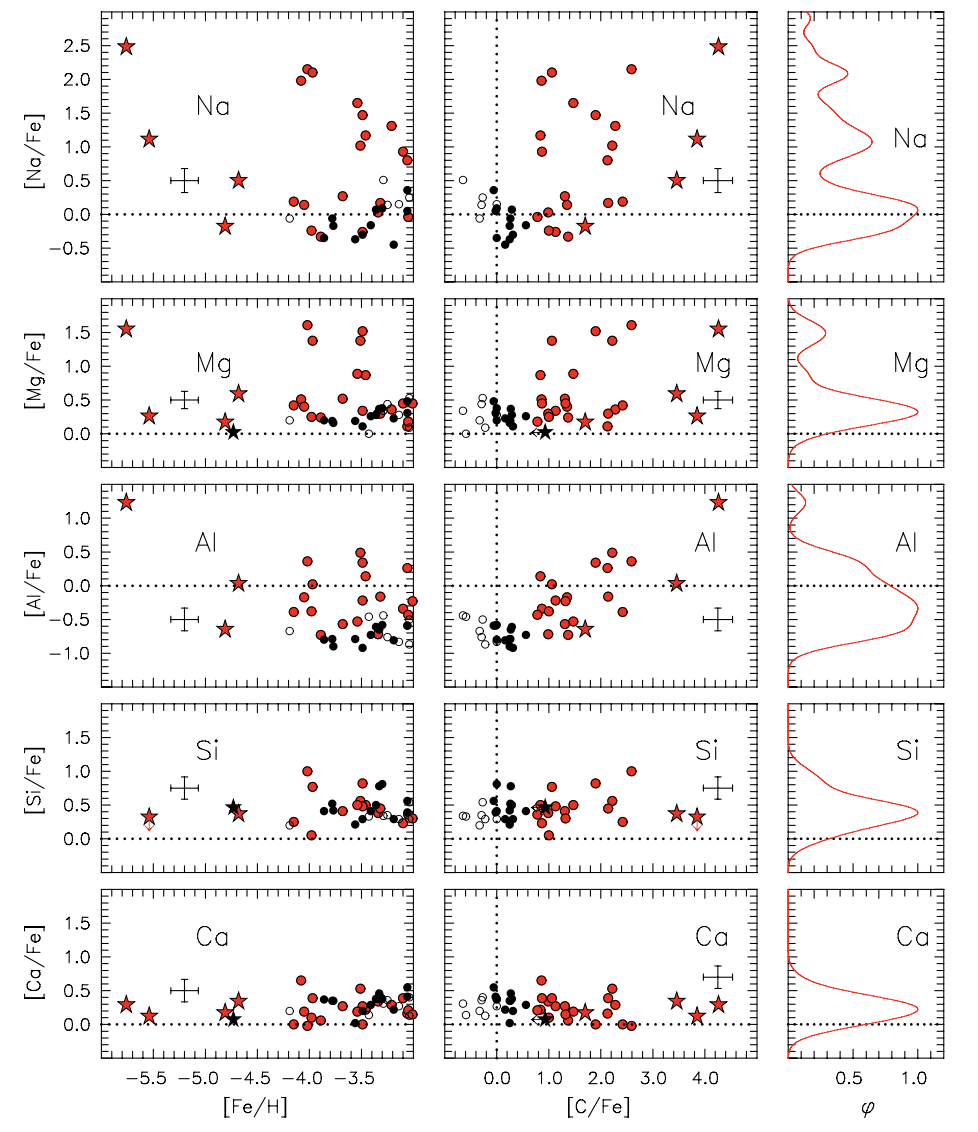
\includegraphics[width=1 \textwidth]{namg}
  \caption{Abbondanze relative degli elementi leggeri Na, Mg, Al, Si e Ca vs [Fe/H] (a sinistra) and [C/Fe] (al centro) per stelle d’alone C-rich e C-normal. La colonna a destra contiene gli istogrammi generalizzati delle abbondanze per le stelle C-rich a sinistra.  
 }
  \label{namg}
 \end{figure}
\

La figura \ref{namg} mostra le abbondanze di [Na/Fe], [Mg/Fe], [Al/Fe], [Si/Fe] e [Ca/Fe] in funzione di [Fe/H] e [C/Fe] per le stelle C-rich e C-normal dell’alone galattico insieme agli istogrammi generalizzati. Le abbondanze di questi elementi contengono informazioni essenziali per la comprensione delle stelle con [Fe/H] $<$ -3.0. Si nota una bassa dispersione in tutti gli elementi per le stelle C-normal mentre è alta per il Na, Mg e Al nelle stelle C-rich. Per il Si e il Ca sembrano esserci basse dispersioni ma per il Si l’abbondanza è stata ricavata analizzando solo una riga per cui sono necessarie ulteriori lavori. Per ultimo si può notare che non tutte le stelle C-rich mostrano grandi sovrabbondanze di Na, Mg e Al ma solo circa la metà. \\
Le figure \ref{cno} e \ref{namg} sono indicative del fatto che le abbondanze riscontrate provengano da materiale parzialmente processato dalla nucleosintesi nelle regioni H-burning che sono soggette anche a He-burning. Quindi suggeriscono la necessità di distinguere le due popolazioni stellari sotto [Fe/H] = -3.0: una C-rich e una C-normal. 




\newpage

\section{Cosmologia Near-Field}

È di fondamentale importanza studiare e interpretare i trend di evoluzione chimica di un determinato sistema sulla base dei processi fisici legati alla nucleosintesi e degli ambienti che ospitano questi processi di arricchimento chimico. In particolare l’osservazione delle stelle di bassa metallicità fornisce una grande quantità di dati sulle abbondanze chimiche relative che sono legate alla formazione delle prime stelle nella galassia. Questi tassi di abbondanze chimiche sono vincolati da molti fattori tra cui la funzione iniziale di massa delle stelle di popolazione III, il tasso di formazione stellare e i prodotti delle supernove.


\subsection{Proprietà delle prime strutture cosmiche}

\paragraph{La natura delle prime stelle} 

Ad oggi nessuna stella di popolazione III è stata osservata. Nonostante siano state scoperte alcune stelle estremamente povere di metalli ([Fe/H] $<$ -5.0), le loro elevate abbondanze di carbonio suggeriscono che siano tra le prime stelle di popolazione II.
L’apparente assenza di stelle di popolazione III è dovuta a difficoltà osservative o esiste una ragione fisica per la quale non si vedono? La natura delle prime stelle è stata ampiamente studiata e dibattuta negli scorsi decenni mentre le simulazioni di questi oggetti si fanno sempre più dettagliate. I principali risultati di queste ricerche sono riportati di seguito.
\subparagraph{Range di massa}

I primi studi sui range di massa delle prime stelle suggerivano masse dell’ordine di 100 M$_{\odot}$, tuttavia le più recenti simulazioni che seguono la formazione della protostella per un periodo maggiore fino alla fase di accrescimento mostrano un quadro più complesso.\\
\cite{hosokawa} hanno simulato la formazione di una stella di 43M$_{\odot}$ fino all’inizio della fase di fusione nucleare. Durante la sua fase di accrescimento, che determina la massa finale della stella di popolazione III, ipotetiche frammentazioni del disco di accrescimento dovute a instabilità gravitazionali, portano alla formazione di stelle di piccola massa. La prima stella tuttavia rimane massiva (decine di M$_{\odot}$) mentre le stelle secondarie possono avere anche masse di circa 1 M$_{\odot}$.  Queste ultime ricerche hanno riaperto la possibilità di osservare le stelle di popolazione III, dati i tempi di vita associati a tali masse ($<$1M$_{\odot}$ corrisponderebbero a tempi di vita $>$ 13 Gyr).\\

La IMF (funzione iniziale di massa) descrive la distribuzione iniziale di massa per una popolazione di stelle ed è di fondamentale importanza per interpretare l’evoluzione delle stelle di pop. III e la formazione delle galassie. A differenza della presente funzione di massa (PDMF), dominata da stelle di piccola massa, la IMF è dominata da stelle massicce. Tuttavia è complicato determinare la IMF a causa della varianza cosmica e di varie difficoltà modellistiche. \cite{Hirano_2014} simulando 100 stelle hanno trovato distribuzioni di massa da 10 a 1000 M$_{\odot}$ . 
Nel contesto cosmologico è prevista l’esistenza di stelle con masse di migliaia di volte quella solare e simulazioni di stelle di pop III con masse 10$^{4-5}$M$_{\odot}$ portano al loro collasso in un buco nero supermassiccio, non contribuendo all’arricchimento chimico, \cite{Hosokawa_2013}. Questi oggetti sarebbero abbastanza luminosi da poter essere osservati direttamente con JWST se la loro esistenza fosse reale. 

\subparagraph{Nucleosintesi delle prime stelle}

Stelle con masse superiori a 8M$_{\odot}$ terminano la loro vita in supernove. In base alla  loro massa e allo stato di rotazione alcune esplosioni portano ad arricchimento chimico mentre altre no. In questo contesto le stelle che muoiono in PINSe (supernove a instabilità di coppia) sono di primaria importanza per l’archeologia stellare infatti stelle di popolazione III non rotanti, con masse $\sim$ 140-260 M$_{\odot}$ esplodono in PINSe. Tuttavia nessuna stella che mostri abbondanze chimiche riconducibili a supernove a instabilità di coppia è stata osservata finora. Le particolari abbondanze chimiche osservate di cui si è discusso nella sezione \ref{abbondanze1} hanno ispirato i più recenti studi teorici che si stanno focalizzando su range di massa inferiori 25-60 M$_{\odot}$, sugli effetti della rotazione sulla nucleosintesi e sui getti atipici delle esplosioni delle supernove. 

\paragraph{La natura delle prime galassie e la formazione delle stelle di piccola massa}
\label{natura_galassie}
Dopo circa 100-200 milioni di anni dal Big Bang, corrispondente a redshift $\sim$ 20 - 30, la formazione delle prime strutture cosmologiche ha inizio dal collasso dei mini-aloni di materia oscura di massa $\sim 10^{6}$ M$_{\odot}$ trascinando la materia barionica (\cite{Greif_2011}). Ogni mini alone ospita una prima stella o più e la sua evoluzione contribuirà all’arricchimento chimico dello stesso. Queste stelle massicce durante la loro breve vita hanno fornito una grande quantità di radiazione ionizzante che ha cambiato le condizioni del gas primordiale circostante. In questa fase della formazione stellare il raffreddamento è dovuto al deuteruro di idrogeno HD mentre nella fase prima era dovuto all’idrogeno molecolare H$_{2}$ e questo comporta una diminuzione della temperatura del gas, quindi alla formazione di stelle meno massicce. È interessante notare che nei mini aloni che non sono stati soggetti ad arricchimento chimico si sia formata una generazione di stelle di popolazione III con masse di circa 10M$_{\odot}$ (\cite{Johnson}). \\
A redshift z $\sim$ 15 una decina di mini aloni si uniscono a formare i cosiddetti “atomic cooling halos” (aloni di raffreddamento atomico) con una massa di materia oscura di $\sim$ 10$^{8}$ M$_{\odot}$.  In questi sistemi i metalli sono presenti e sono convogliati dal fondersi dei mini aloni che ospitavano stelle di popolazione III esplose in supernove. 
Questi aloni di raffreddamento atomico a causa della loro massa elevata, della metallicità in grado di ospitare la formazione delle stelle di popolazione II e della capacità di non disgregarsi in seguito a supernove possono essere considerati le prime galassie. \\
Secondo altre teorie alcune delle prime stelle di piccola massa potrebbero essersi già formate nei mini aloni. L’arricchimento metallico dell’alone, durante il processo esplosivo di una supernova, avviene su lunghezze scala che influenzano gli aloni circostanti anche se questi non contengono a loro volta stelle di popolazione III. Questi lavori mostrano come l’arricchimento metallico delle prime galassie provenga da diverse fonti e in modi così disomogenei (\cite{Wise}). Questo processo ha dato inizio alla formazione delle stelle di popolazione II poiché le prime galassie hanno fornito le condizioni ottimali per la formazione delle prime stelle di bassa metallicità di piccola massa M$<$1M$_{\odot}$.  La disponibilità di metalli ha reso possibile la formazione di polveri e il conseguente raffreddamento dovuto ad esse. Anche se le modalità della formazione delle prime stelle di piccola massa non sono ben definite, esiste un concetto di metallicità critica. Una notevole frammentazione del gas avviene sopra la metallicità critica e in questi ambienti è possibile la formazione delle stelle di piccola massa come risultato dell’espulsione dalla dinamica di N-corpi prima che queste protostelle raggiungano la massa termica di Jeans. Questi corpi sarebbero oggi osservabili nella Via Lattea o nelle sue galassie nane satelliti. Mentre al di sotto della metallicità critica solo le stelle massicce,  quindi con tempi di vita brevi, sarebbero in grado di formarsi.
Per la formazione delle stelle di piccola massa si considerano due diversi metodi per l’individuazione della metallicità critica, uno basato sul raffreddamento legato alle righe di struttura fine dell’atomo e il secondo sul raffreddamento dato dalle polveri. Le metallicità critiche trovate rispettivamente sono Z$_{crit}$ $\sim$ 10$^{-3.5}$ Z$_{\odot}$ e Z$_{crit}$ $\sim$ 10$^{-5}$ Z$_{\odot}$. La frammentazione, quindi la formazione delle stelle di piccola massa, avviene in entrambi i casi.
Tuttavia molti dettagli sui processi di frammentazione indotti dai due tipi di raffreddamento rimangono da approfondire. 
%Tuttavia  un metodo per testare come questo meccanismo influenza la formazione delle stelle di popolazione II è comparare le predizioni teoriche con le abbondanze chimiche rilevate per le stelle più metal-poor conosciute. Dopo tutto queste sono le stelle che si assume si siano formate per prime nelle galassie e possono fornire importanti informazioni sul loro meccanismo di formazione. \\%
Secondo \cite{Frebel2007}  tutte le stelle estremamente metal poor che si sono formate attraverso il raffreddamento dovuto alle righe CI e OII dovrebbero mostrare abbondanze di carbonio e/o ossigeno in eccesso rispetto alla metallicità critica della rispettiva riga. Finora sembra che quasi tutte le stelle [Fe/H] $<$ - 3.0  rispettino ancora questa condizione. 


\subsection{Origini e interpretazioni delle abbondanze chimiche per stelle [Fe/H] $<$ -3.0}
\label{crich_origin}

\paragraph{Origini delle stelle C-rich}
Attualmente nessuna ipotesi riesce a spiegare completamente le origini delle stelle C-rich con [Fe/H] $<$ -3.0 ma sono stati considerati diversi scenari che probabilmente hanno avuto un ruolo nella formazione di queste stelle tra cui:
\begin{itemize}

\item Transizioni tra i livelli energetici di struttura fine delle righe di CII e OI sono responsabili del raffreddamento durante la formazione di queste stelle. Gas C-rich / O-rich hanno formato stelle, tramite la frammentazione, in tempi scali più brevi rispetto ad altre zone meno C-rich/O-rich (\cite{Frebel2007}). 
\item Stelle supermassice rotanti (100 $<$ M $<$ 300 M$_{\odot}$) ( \cite{Fryer}). In questi range di massa la rotazione induce un mescolamento del carbonio e dell’ossigeno dal nucleo He-burning alla shell H-burning.  Questo porta ad una produzione maggiore di C, N, O osservabile sulle superfici stellari.
\item supernove di tipo II mixing and fallback (M $\sim$ 10 - 40M$_{\odot}$): basse energie di esplosione di supernove eiettano il materiale principalmente dalle regioni più esterne che sono arricchite di elementi leggeri e solo una piccola parte di elementi pesanti che si sono formati più all’interno nella stella. Durante l’esplosione avviene un mescolamento interno in una regione fuori dal taglio di massa dove è iniziata l’espansione. La maggior parte della materia mescolata ricade verso il nucleo mentre una piccola parte viene espulsa, \cite{iwamoto}.

\item supernove multiple di tipo II con ricadute di materiale e/o getti relativistici (M $\sim$ 10 - 40 M$_{\odot}$) supernove di energie “normali” ($\sim$ 10$^{51}$ erg) in combinazione con quelle di basse energie ($<$ 10$^{51}$ erg). Un getto relativistico indotto da un’ esplosione di supernova di 40M$_{\odot}$ porta alla ricaduta del materiale più interno che diminuisce la quantità di elementi più pesanti (Fe) espulsi dal getto rispetto a quelli più leggeri (C). \cite{Tominaga}

\item stelle rotanti massicce ($\sim$ 60M$_{\odot}$) e intermedie ($\sim$ 7M$_{\odot}$): la rotazione induce un aumento di CNO e un eccesso di $^{13}$C, Na, Mg, Al nel materiale espulso dai venti stellari. \cite{Meynet}.

\end{itemize}

\paragraph{Limiti delle interpretazioni}
\label{limiti}

Nell’interpretazione delle abbondanze delle stelle con le più basse metallicità sorgono diversi problemi osservativi, teorici e altri. 
I problemi osservativi consistono principalmente nella difficoltà di ottenere ampio numero di abbondanze chimiche,  un esempio è la stella di \cite{keller} con [Fe/H] $<$ -7.2.
Per questa stella è stato possibile determinare solo quattro abbondanze chimiche a causa della loro bassissima presenza e ciò ha reso più complicato trovare un modello accettabile.\\ Inoltre anche errori sistematici legati all’uso dei modelli 1D/LTE per le abbondanze chimiche rispetto a quelli 3D/NLTE hanno ampliato il margine tra modello e osservazione. In particolare, come in figura \ref{1d3d}, le correzioni per C, N e O possono eccedere anche di 0.5 dex e influenzare in modo significativo i modelli. Infatti per questa stella \cite{ishigaki} trovano progenitori di 25M$_{\odot}$  e 40M$_{\odot}$  mentre Keller et al. (figura \ref{keller2}) di 60 M$_{\odot}$.
Similmente per la stella di Nordlander si trovano modelli di best fit di progenitrici di 11.2 M$_{\odot}$  e 50M$_{\odot}$, figura \ref{nordlander2}.\\
I problemi teorici riguardano la moltitudine di parametri liberi che hanno i modelli di nucleosintesintesi come le energie di esplosione, il taglio di massa, la rotazione stellare, i processi di nucleosintesi…
Le esplosioni vengono trattate sfericamente semplificando così il modello ma introducendo altri errori sistematici. Tutti questi parametri impediscono previsioni delle masse stellari e quindi i modelli vengono fatti combaciare a posteriori con le osservazioni.  
Altri problemi riguardano per esempio i processi di mescolamento eterogeneo del gas di formazione stellare che portano a diluizioni locali differenti e quindi pattern di abbondanze diverse tra una generazione di stelle e quella successiva ( \cite{Ritter}). Oppure l’accrescimento di materiale interstellare durante la vita della stella può portare ad alterazioni delle abbondanze come anche l’inquinamento da una compagna binaria (\cite{Hattori}). \\
\cite{principale} hanno riassunto nella tabella \ref{table} le abbondanze chimiche vincolanti per distinguere le proprietà delle stelle di popolazione III e le nucleosintesi delle supernove. 


\begin{table}[h!]
\centering
\caption{abbondanze chiave che vincolano le stelle di popolazione III e le nucleosintesi delle supernove}
\label{table}
\resizebox{\textwidth}{!}{%
\begin{tabular}{lll}
\hline
\multicolumn{1}{l}{\textbf{abbondanza}} & \textbf{tasso (dex)} & \multicolumn{1}{l}{\textbf{proprietà della pop. III}}                                                                       \\ \hline
{[}C/Fe{]}                               & $>$1.0               & \begin{tabular}[c]{@{}l@{}}Supernova di collasso nucleare "mixing and fallback"\\ stella massiccia, rotante, Z=0\end{tabular} \\
{[}C/N{]}                                & $<$0.0               & stella massiccia, rotante, Z=0                                                                                                \\
{[}Na, Mg, Al/Fe{]}                      & $>$1.0               & rotante, Z=0, Supernova di collasso nucleare "mixing and fallback"                                                           \\
{[}$\alpha$/Fe{]}                               & $\sim$ 0.4           & supernova di collasso nucleare                                                                                               \\
{[}Ca/Fe{]}                              & $>$1.0               & PISNe                                                                                                                        \\
{[}Zn/Fe{]}                              & $>$0.5               & Supernova di collasso nucleare con alte energie di esplosione                                                                \\ \hline
\end{tabular}%
}
\end{table}

\paragraph{Influenza della rotazione}

Molti modelli sono stati ipotizzati sulle origini delle stelle C-rich nella sezione \ref{crich_origin} tra cui il più promettente e il più studiato riguarda il modello di supernove di tipo II "mixing and fallback". In queste supernove a basse energie di esplosione ($<$ 10$^{51}$ erg) solo gli strati più esterni della stella che contengono gli elementi più leggeri vengono espulsi dai getti. Gli elementi più pesanti risiedono negli strati più interni e ricadono nel buco nero che si forma successivamente l’esplosione. Solo una piccola parte degli elementi pesanti viene espulsa dai getti determinando il basso arricchimento metallico da questi elementi. Questo potrebbe spiegare le abbondanze delle stelle più povere di metalli ([Fe/H] $<$ - 4.5 ) che si conoscono (sezione \ref{povere}) comprese le stelle di Keller e di Nordlander. 
\ Simulazioni di \cite{Stacy} supportano l’idea che le stelle di popolazione III potrebbero essere rotanti. Questo ha un notevole impatto sull’evoluzione della stella ma soprattutto sulla nucleosintesi stellare. La sostanziale differenza tra i modelli rotativi e quelli delle supernove "mixing and fallback" è la differente regione della stella di popolazione III che produce l’arricchimento della progenie. Nel modello rotante l’arricchimento è prodotto dagli strati più esterni tramite mescolamento dovuto alla rotazione, mentre nel secondo modello è dovuto a tutti gli strati fuori dal nucleo che si mescolano tra di loro durante l’esplosione di supernova. Il silicio e il calcio sono elementi che sono prodotti negli strati intermedi di una stella e la rilevazione di queste abbondanze permetterebbe di discernere al meglio il modello da usare. \

Si potrebbero avere risultati interessanti in quest’area considerando un modello che tenga conto dell’influenza reciproca di diversi meccanismi di esplosione, tra tutti una combinazione del modello “mixing and fallback” e quello rotante.

\paragraph{Legame tra le popolazioni C-rich e C-normal }

Nella sezione \ref{natura_galassie} si è discusso dei processi di raffreddamento delle polveri e quelli dovuti alle righe CI e OII che potrebbero aver portato alla formazione delle popolazioni C-rich e C-normal. È interessante approfondire le cause dei due processi. 
\cite{Norris_2013} considerano un semplice scenario nel quale le stelle di popolazione II di piccola massa si siano formate da nubi con elevate abbondanze di carbonio e ossigeno rispetto ad altri metalli più pesanti.
D’altra parte una frazione delle stelle di popolazione III non ha prodotto grandi abbondanze di carbonio probabilmente a causa delle energie di esplosione più canoniche o a rotazioni stellari minori. Il gas espulso da questo tipo di supernove ha abbondanze simili a quelle solari e subisce il raffreddamento delle polveri una volta superata la metallicità critica associata. 
\cite{Cooke_2014} hanno considerato la formazione delle stelle c-rich usando simulazioni di modelli cosmologici di arricchimento chimico nei mini aloni. Hanno trovato che le supernove "mixing and fallback", di basse energie, associate ad elevate abbondanze di carbonio, non hanno abbastanza energia da espellere il gas dai mini aloni. La stella di popolazione II sarebbe così una stella C-rich. D’altra parte supernove di tipo PISNe avrebbero abbastanza energia da espellere tutto il gas dal mini alone. Ciò precluderebbe la formazione delle stelle con abbondanze riconducibili a una tale supernova ma anche ad un'eventuale stella C-rich. In generale i pattern di arricchimento dei mini aloni si hanno ipotizzando l’energia di esplosione iniziale e la IMF.  Queste simulazioni sono in grado di spiegare come si distribuiscono le stelle CEMP-no con [Fe/H] $<$ -3.0 e la maggior frequenza di stelle C-rich al diminuire della metallicità.





\subsection{Cosmologia Near Field vs Far Field}



I risultati ottenuti dagli studi near-field si basano sull’assunzione che le stelle più povere di metalli si formino da nubi di bassa metallicità entro il primo miliardo di anni dal Big Bang. Questa ipotesi è supportata dalle stelle arricchite da elementi derivanti dal processo r che mostrano tempi scala di 13-14 Gyr e [Fe/H] $\sim$ -3.0. 
Tuttavia è importante verificarla anche osservando direttamente i primi sistemi gassosi ad alti redshift e il loro contenuto metallico. 
200 misurazioni delle metallicità per i sistemi Lyman-$\alpha$ smorzati (DLA) a redshift z  $\sim$ 2-5 sono state identificate lungo la linea di vista di un dato quasar da \cite{Rafelski}. Questi dati mostrano in media un lento decremento della metallicità al crescere del redshift. 
\cite{Fumagalli} hanno studiato i sistemi Lyman limit (LLSs) lungo due quasar a redshift z$\sim$ 3.4 e $\sim$ 3.1 e rilevato metallicità di Z$<$10$^{-4.2}$Z$_{\odot}$ e Z$<$10$^{-3.8}$Z$_{\odot}$. Non è chiaro se i sistemi LLSs abbiano formato le attuali stelle di bassa metallicità che si osservano attualmente. 
Questi redshift implicano un’ epoca di 2 Gyr dopo il Big Bang e potrebbero rappresentare i primi sistemi che hanno ospitato le stelle di popolazione II. Tuttavia servono sistemi a redshift più alti per poterli confrontare con i dati della cosmologia near field.  
Un caso più estremo è quello presentato da \cite{Simcoe} che hanno trovato un sistema gassoso a z $\sim$ 7 ($\sim$ 800 Myr) lungo il quasar ULAS J1120+0641. La metallicità ha un limite superiore di Z$<$10$^{-3.0}$Z$_{\odot}$ se il gas è diffuso e Z$<$10$^{-4.0}$Z$_{\odot}$ se è una proto galassia gravitazionalmente legata.

\paragraph{Abbondanze chimiche delle nubi di idrogeno neutro ad alto redshift.}
%Abbondanze nei sistemi gassosi ad alti redsfhit}

Nei sistemi DLA l’abbondanza di numerosi elementi chimici può essere ottenuta osservando tali sistemi lungo la linea di vista di un quasar. Uno dei principali studi del settore e' quello di \cite{Cooke_2011} in cui gli autori hanno stimato le densità di colonna per undici elementi. In un campione di 21 oggetti a redshift 2$<$z$<$ 4 hanno trovato tre sistemi di bassa metallicità in un intervallo di metallicità -3.5$<$[Fe/H] $<$-3. Inoltre, le abbondanze per C, O sono consistenti con i valori determinati per le stelle dell’alone galattico.

Tuttavia \cite{Becker} hanno riportato le abbondanze per C, O, Si e Fe per sistemi sub-DLA a redshift z=6.3 quindi sistemi a redshift maggiori rispetto Cooke et al (2011) estendendo il loro set di dati e non hanno trovato variazioni significative delle abbondanze rispetto al redshift (figura \ref{dla}). Per i quattro sistemi a redshift 4.7 $<$z$<$ 6.3 hanno trovato valori medi di [C/Fe] = $+0.17 \pm 0.07$ and [O/Fe] = $+0.50  \pm 0.05$ in ottimo accordo con i valori per le stelle di più bassa metallicità dell'alone.

Quindi nei sistemi sub-DLA ai più alti redshift le abbondanze di carbonio e ossigeno sono consistenti con quelle stelle C-normal dell’alone. Secondo gli autori, se le stelle C-rich riflettono le abbondanze delle nubi che le hanno generate, allora tali abbondanze non sono più comuni a redshift z $\sim$ 6. Questo porta ad ipotizzare che le stelle C-rich si siano formate molto prima rispetto alle C-normal.
Tuttavia il campione di dati è chiaramente troppo piccolo per permettere tali conclusioni anche perché non è possibile sapere quale regione del sistema DLA viene osservata lungo la linea di vista.


\begin{figure}[htp!]
\center
  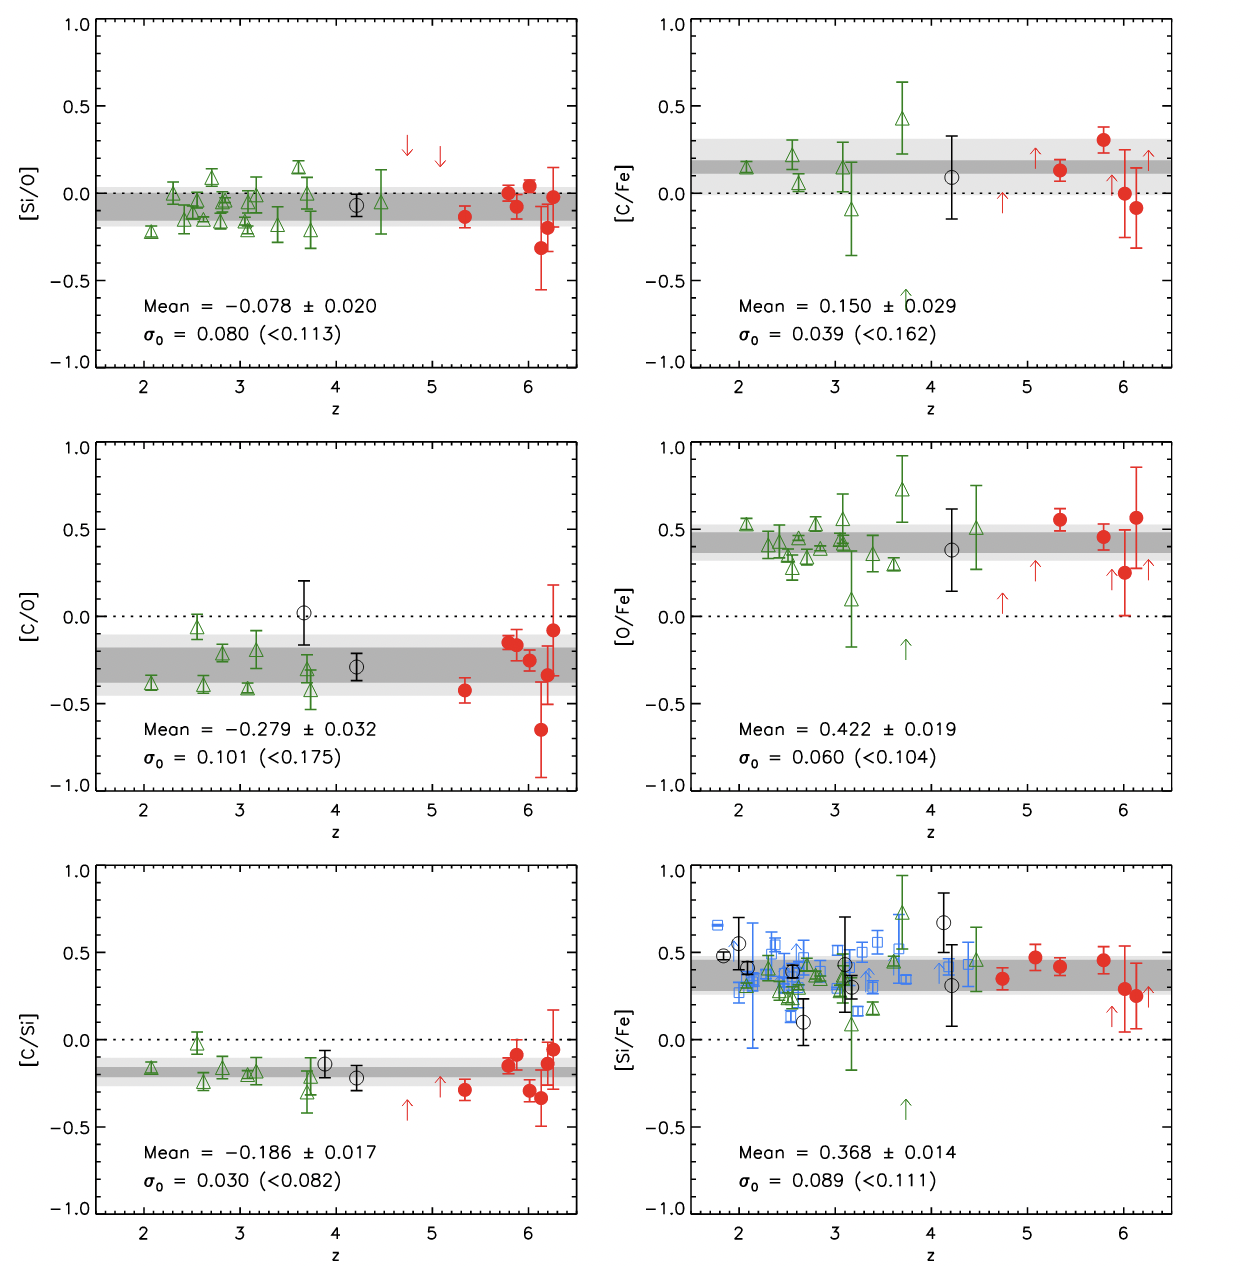
\includegraphics[width=1 \textwidth]{Becker}
  \caption{ Abbondanze relative per sistemi DLA e sub-DLA. In tutti i casi le abbondanze sono state ricavate tramite le densità di colonna. I marker e i diversi colori indicano la diversa provenienza dei dati. Per ogni pannello è fornito il valore medio e un’incertezza di 1$\sigma$ calcolati sui dati provenienti da tutti i lavori. Stime sugli intervalli di confidenza $\sigma_{0}$ e 1$\sigma$ sono riportate in figura con bande rispettivamente di colore grigio scuro e chiaro e segnate in ogni pannello. \cite{Becker}
}
  \label{dla}
\end{figure}





\newpage









\section{Prospettive future}




Gli ultimi decenni sono stati molto proficui nell’analizzare la Via Lattea in particolare nel suo contenuto stellare, nella popolazione dei suoi satelliti e nella storia della sua formazione. La survey SMSS ha portato alla scoperta delle stelle alle più basse metallicità tra cui quelle di Keller e di Nordlander. 
Un progresso significativo è stato effettuato anche nelle simulazioni delle prime stelle e delle prime galassie con particolare attenzione all’evoluzione chimica e alla formazione galattica. Nonostante questi progressi le domande aperte sono numerose. In particolare sui limiti della metallicità di una stella, sulla frazione di stelle c-rich alle più basse metallicità, sull’arricchimento chimico da supernove e soprattutto sull'osservabilità di una stella di popolazione III. I telescopi più avanzati non hanno ancora la potenza osservativa necessaria da poter rilevare le prime stelle e neanche la prossima generazione di telescopi riuscirà molto probabilmente a trovarle. Tuttavia i futuri telescopi in particolare il "Giant Magellan Telescope" (GMT) potrebbe portare significativi progressi al campo dell’archeologia stellare e delle galassie nane ampliandone il catalogo e vincolando le simulazioni con nuovi dati. Il GMT con i sui sette specchi per un diametro complessivo di $\sim$ 25 m e lo spettrografo G-CLEF permetteranno di ottenere spettri delle stelle più metal poor dell’alone e delle galassie nane con una risoluzione fino a R $\sim$ 100000. Il GMT monterà anche uno spettrografo a bassa risoluzione per indagare le stelle candidate. \\
Anche il "Extremely large telescope" (ELT) con il suo specchio primario di $\sim$ 40 m permetterà osservazioni delle galassie dai più alti redshift fornendo così informazioni complementari alla cosmologia near-field.
Il JWST purtroppo non ha un potere risolutivo sufficiente per osservare singole stelle di popolazione III ma permetterà osservazioni ai più alti redshift delle primissime galassie e con una buona dose di fortuna anche i primi ammassi stellari che si sono formati nell’universo tramite lensing gravitazionale. \\
Le osservazioni delle stelle alle più basse metallicità forniscono un potente strumento per cercare le prime stelle ma non possono fornire un'informazione diretta su come si siano formati i sistemi che le ospitano. Simulazioni cosmologiche sono necessarie per comprendere la formazione di queste prime strutture. Quindi il progresso della cosmologia near field deve avvenire di pari passo allo sviluppo delle simulazioni cosmologiche. 









\newpage
\
\printbibliography

\end{document}
